\documentclass[12pt]{article}
\usepackage[utf8]{inputenc}
\usepackage{amsmath}
\usepackage{amssymb}
\usepackage{multicol}
\usepackage{fullpage}
\usepackage{bera}
\usepackage{xcolor}
\usepackage{hyperref}
\usepackage{graphicx}
\graphicspath{ {images/} }

\setlength{\parindent}{0pt}

\begin{document}
\begin{flushleft}
{\footnotesize Pontificia Universidad Católica de Chile\\
Departamento de Ciencia de la Computación\\
Computación: Ciencia y Tecnología del Mundo Digital\\
}
\begin{center}
{\huge\bf Tarea Chica 3: Máquinas de Turing}\\ \vspace{0.5cm}
Profesor Denis Parra \\

\rule{\linewidth}{0.1mm}
\end{center}
\end{flushleft}

\section*{Explicación y funcionamiento de la máquina }

Para poder entender el funcionamiento de la máquina es necesario entender lo que realizó el algoritmo desde que recibió el input hasta que ejecutó la respuesta. En esta sección se explicará de manera general el funcionamiento de cada estado ya que posteriormente se verá una explicación mas profunda. \\

En primer lugar, la máquina recibe un input del cual tiene como objetivo verificar si es que es una secuencia consecutiva de números binarios ordenados de forma decreciente y separados por un gato. La máquina funciona mediante dos cintas, las cuales una se encargará de mantener y 'limpiar' el input, mientras que la otra irá realizando la resta desde el primer número del input. Tras cada resta se verificará si este número es efectivamente el número que sigue, revisándolo con el número que se encuentra en la primera cinta. El proceso se va realizando periódicamente hasta que llegue al final de la cinta o de lo contrario, al verificar que el valor de la primera cinta con el de la segunda cinta sean distintos en algún paso de la máquina, provocará que sea rechazada automáticamente. Para entender de manera más específica como lo hace la máquina se verá paso a paso el funcionamiento de la máquina mediante imágenes ilustrativas. \\

\begin{enumerate}
\item \textbf{Replicación primer número del input y posicionamiento} \vspace{0.2cm}\\
    Tras recibir el input se sobrescribe el primer número dado en la segunda cinta (desde el que comienza el input hasta el \text{\#} ). Tras escribir el primer número la cinta 1 se mantiene en su posición (\text{\#}) y la segunda cinta se prepara para restar. Lo podemos evidenciar en esta imagen.\\
    \begin{figure}
        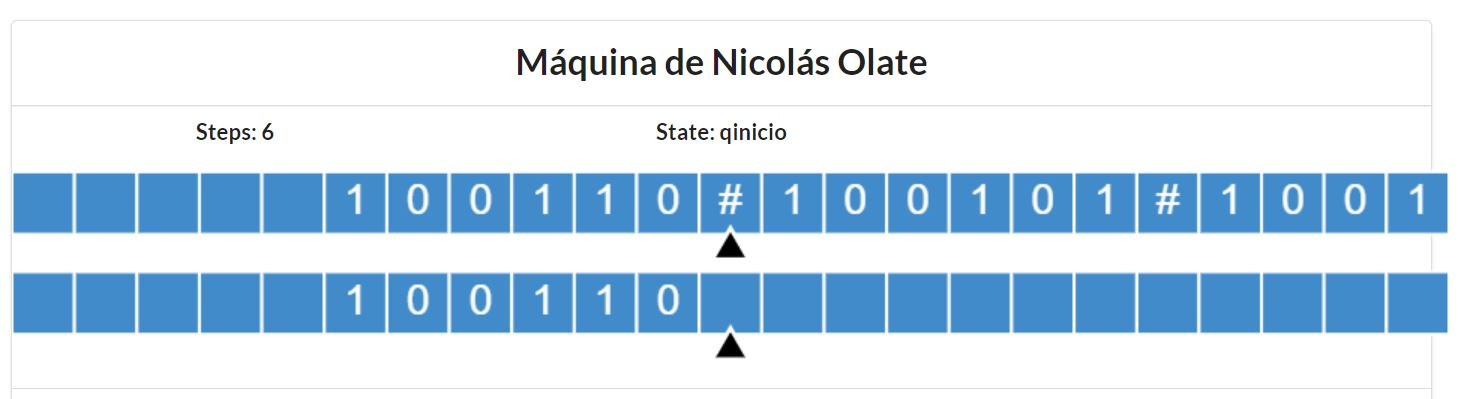
\includegraphics[width=0.7\textwidth]{imagenes/PASO 1.JPG}
        \centering
        \caption{Paso 1}
        \label{fig:paso1}
    \end{figure}
\newpage

\item \textbf{Restar número} \vspace{0.2cm}\\
    Ya con la cinta 2 posicionada se procede a restar una unidad en binario. Para esto se generan 2 casos: 
    \begin{itemize}
	    \item Que simplemente el primer número sea un $1$, a lo que se restará en una unidad (el $1$ pase a $0$) y se reescriban los números anteriores.
	    \item El primer número a restar sea un $0$, lo que se procede a transformar el número en un $1$ (resta en binarios). Tras esto el número siguiente de derecha a izquierda se le aplicará el mismo procedimiento inicial (hasta que el número a restar sea un $1$) repitiendo el procedimiento, obteniendo el nuevo número.  
        \end{itemize}
    Esto lo podemos evidenciar en el siguiente ejemplo que usa ambos casos:
     \begin{figure}[h]
        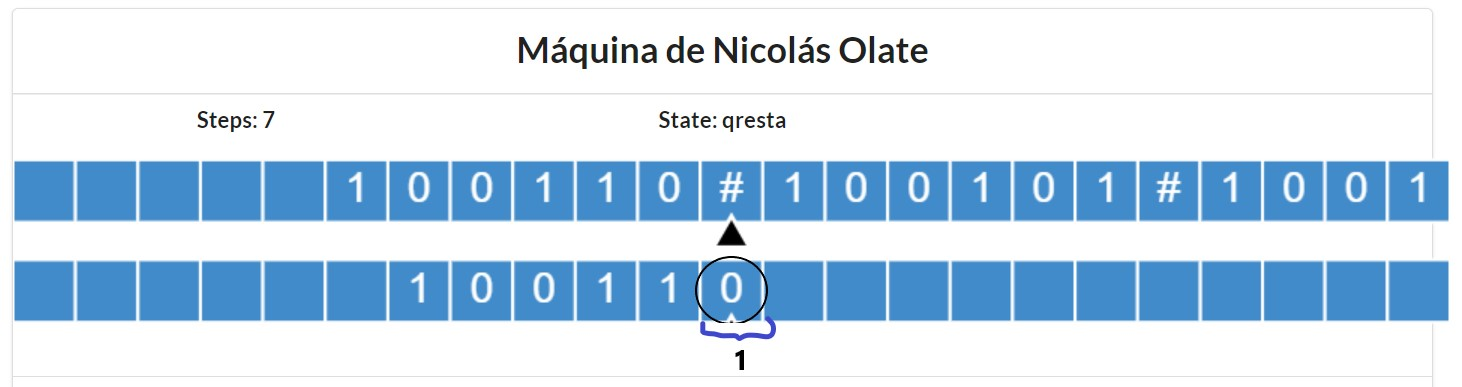
\includegraphics[width=0.7\textwidth]{imagenes/PASO 2.1.jpg}
        \centering
        \caption{Inicio paso 2}
        \label{fig:paso 2.1}
    \end{figure}
    
    Se aplica el segundo caso mostrado cambiando el $0$ por un $1$. Se vuelve a ejecutar el proceso.
    
    \begin{figure}[h]
        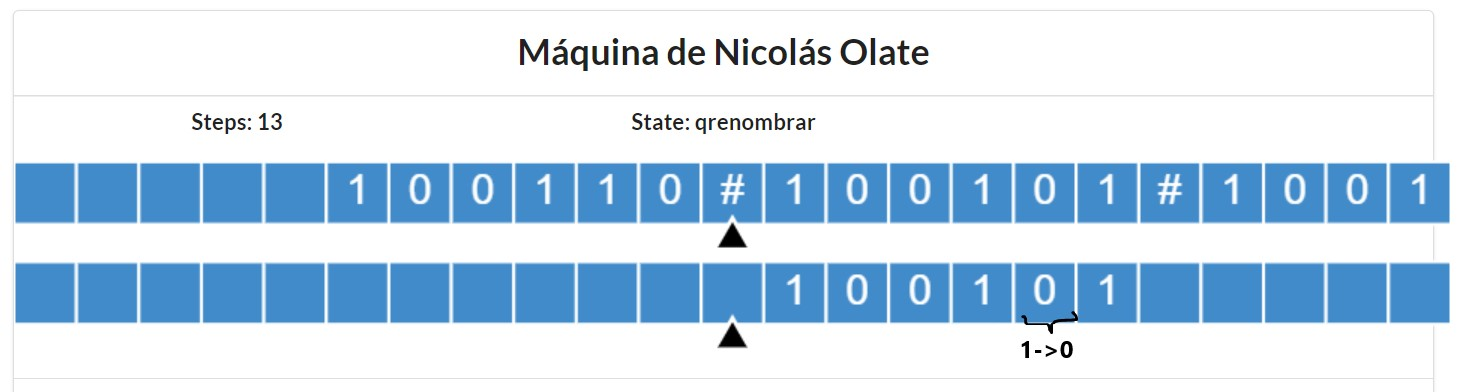
\includegraphics[width=0.7\textwidth]{imagenes/PASO 2.2.jpg}
        \centering
        \caption{Finalización paso 2}
        \label{fig:paso 2.2}
        
    \end{figure}
    \newpage
    Tras repetir el proceso se ve que el siguiente número en el cabezal será un $1$, aplicando el primer caso presentado, este se transforma a un $0$ y se repiten los números.

\item \textbf{Limpiar valores, verificación y repetición del proceso} \vspace{0.2cm}\\
    Tras obtener el número siguiente en la sucesión, se debe verificar si efectivamente es el número según el input dado (cinta 1). Antes de verificar esto, se realizará el bonus correspondiente en el que agregaremos un paso en 'limpiar los valores' para no tener problema con el largo del número binario. Para lograrlo se eliminarán todos los $0$s que que se encuentran antes del primer $1$ dejando los números de igual largo. Esto se verifica con el siguiente ejemplo:
    \begin{figure}[h]
        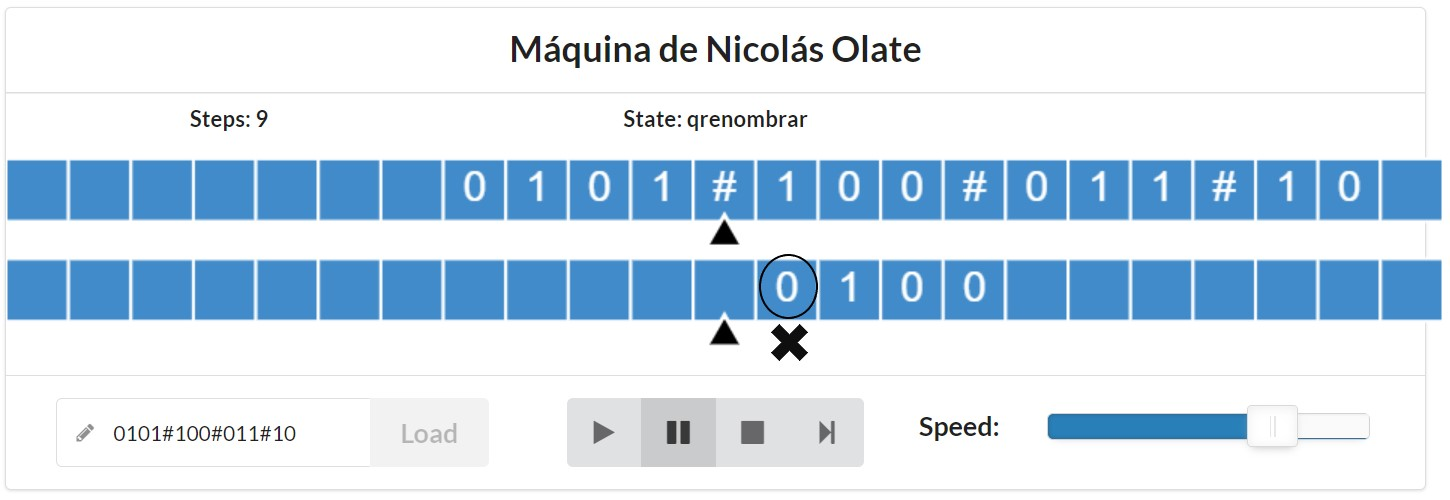
\includegraphics[width=0.7\textwidth]{imagenes/PASO 3.1.jpg}
        \centering
        \caption{Limpieza de datos}
        \label{fig:paso 3.1}
    \end{figure}
    
    Luego de la limpieza de datos se procede a verificar entre el número entregado por el input (cinta 1) y el valor real obtenido (cinta 2) si es que efectivamente poseen el mismo valor. Si es que no tienen algún número igual la máquina lo rechazará (rejected), mientras que si son todos iguales la máquina seguirá su curso. Lo vemos en los siguiente ejemplos:
     \begin{figure}[h]
        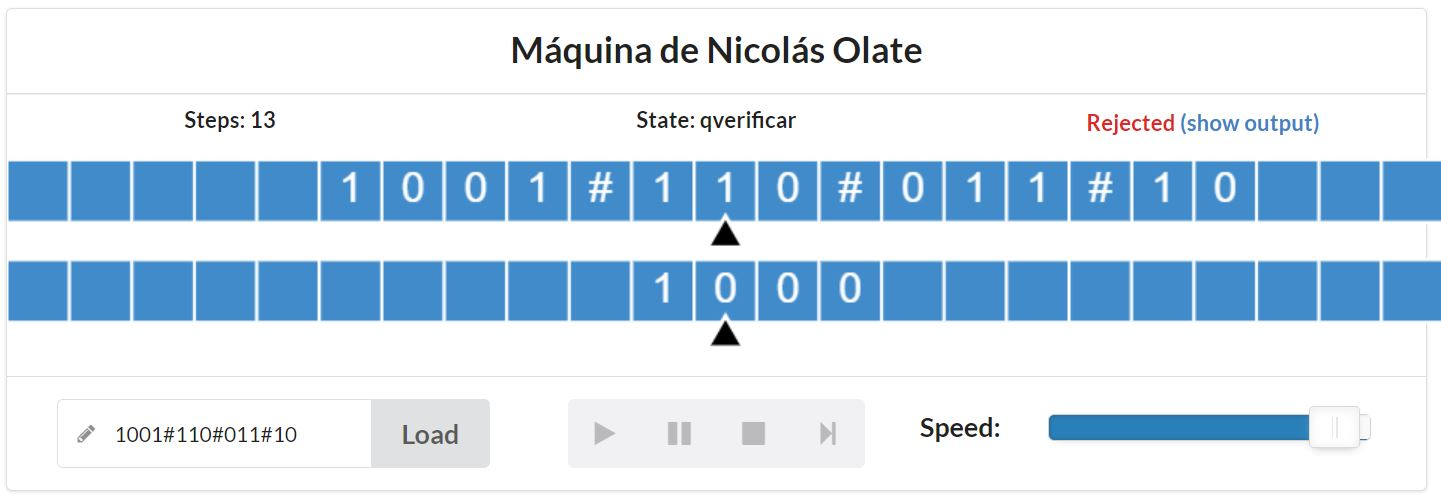
\includegraphics[width=0.7\textwidth]{imagenes/PASO 3.2.JPG}
        \centering
        \caption{Ejemplo de error}
        \label{fig:paso 3.2.1}
    \end{figure}
    \newpage
    El número dado en el input no corresponde a lo que pedían (sucesión decreciente) por lo que la máquina lo rechaza. Mientras que en el siguiente ejemplo se cumplen las condiciones por lo que sigue funcionando la máquina.
    
    \begin{figure}[h]
        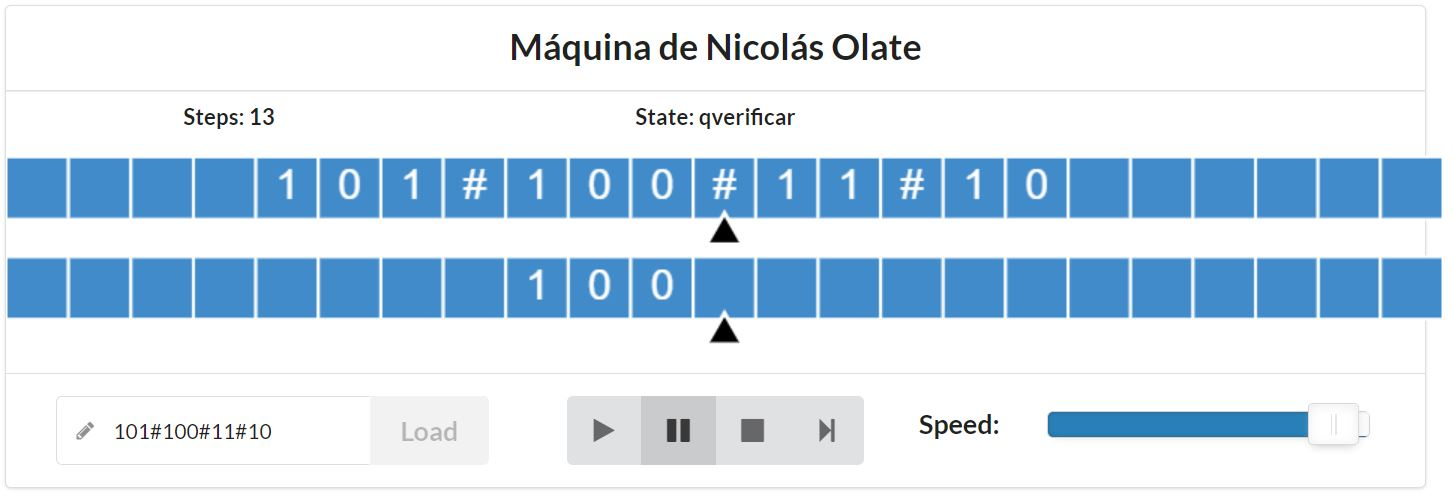
\includegraphics[width=0.7\textwidth]{imagenes/PASO 3.2.2.JPG}
        \centering
        \caption{Ejemplo máquina que sigue funcionando}
        \label{fig:paso 3.2.2}
    \end{figure}
    Finalmente, tras verificar que si era este número su antecesor, realizamos el mismo proceso (restando $1$) al número obtenido, y volvemos a revisarlo, esta vez con el número siguiente en la cinta 1. Esto se hace para todos los números hasta que la cinta 1 se le acaba el input, verificando que si se cumple la secuencia de números retornando verdadero (Accepted). Esto se ve a continuación:
    \begin{figure}[h]
        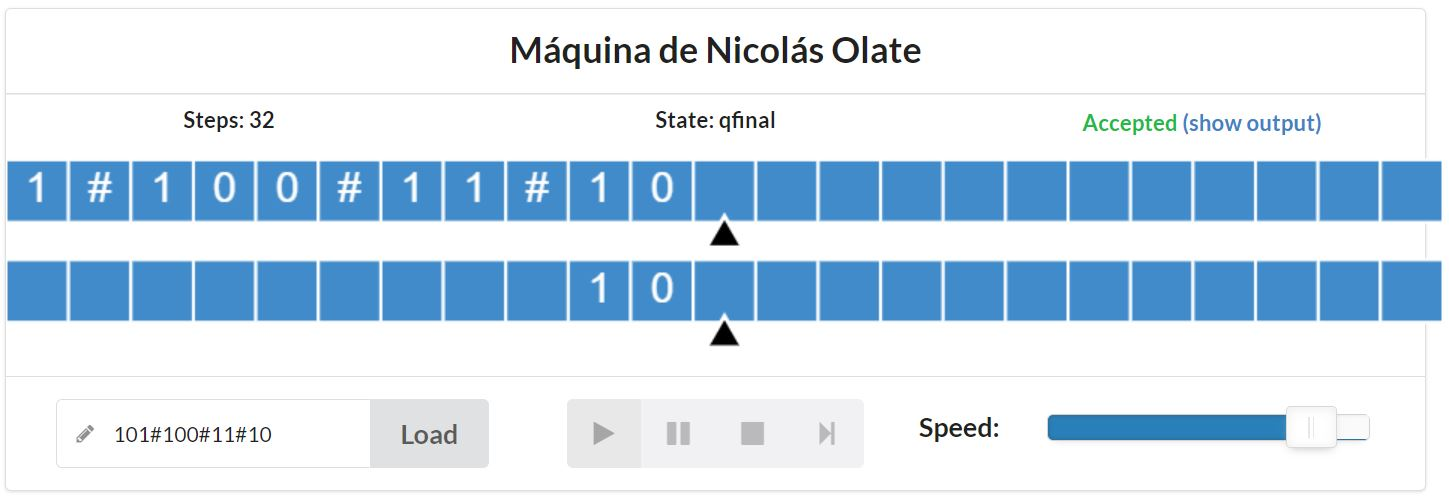
\includegraphics[width=0.7\textwidth]{imagenes/PASO 3.3.JPG}
        \centering
        \caption{Ejemplo máquina que retorna verdadero}
        \label{fig:paso 3.3}
    \end{figure}
\end{enumerate}

\section*{Definición formal para $Q, q_{0}, \Gamma, F$}
En esta esta sección definiremos, los valores $Q, q_{0}, \Gamma, F$ que aparecen en una máquina de Turing (con ayuda del enunciado de la tarea). Estos conceptos se definen formalmente en la máquina de Turing según la tabla mostrada a continuación:
    \[
    \begin{array}{|c|c|}
    \hline
         \text{Símbolo} & \text{Descripción}  \\ \hline
         \text{$Q$} & \text{Conjunto de estados} \\
         \text{$q_{0} \in Q$} & \text{Estado inicial de la máquina}\\
         \text{$\Gamma$} & \text{Alfabeto de la máquina} \\
         \text{$F \subseteq Q$} & \text{Conjunto de estados de aceptación} \\
         \hline
    \end{array}
    \]\\
    Para el caso de la máquina de Turing creada tenemos que:
    \begin{itemize}
        \item $Q = \{q_{inicio}, q_{resta}, q_{renombrar}, q_{arreglar1}, q_{arreglar2}, q_{verificar}, q_{final}\}$
        \item $q_{0} = q_{inicio}$
        \item $\Gamma = \{1 , 0, \text\# \} $
        \item $F = \{ q_{final} \}$ 
    \end{itemize}
    

\section*{Descripción de estados que componen $Q$}
En esta parte hará un análisis mas detallado de los estados que componen la máquina en los que se mencionarán las condiciones para que pase a ese estado, las acciones que realiza la máquina en ese estado y los estados los cuales puede pasar la máquina.
\begin{enumerate}
    \item {\large $q_{inicio}$} \vspace{0.2cm}\\
    Este estado al ser el estado inicial, no se requieren condiciones para que cambie de estado ya que aquí comienza una vez entregado el input. \\
    Este estado tiene como función sobrescribir en la cinta 2 el primer número entregado en el input (desde que comienzan los números hasta el primer \#). Por lo que si recibe un $0$ en la cinta 1, este lo mantiene en la cinta 1 y lo reescribe en la cinta 2. Tras esto avanzan al siguiente número hacia la derecha. Este proceso se realiza de igual manera cuando la cinta 1 recibe un $1$. \\
    Esto finaliza cuando la cinta 1 llega al \# (momento en que se termina el primer número) en el cual la máquina pasa al estado  $q_{resta}$.\\
    \item {\large $q_{resta}$} \vspace{0.2cm}\\
    Existen 2 condiciones para pasar al estado $q_{resta}$. Una de ellas es desde el estado inicial ($q_{inicio}$) en la cual surge ya que se terminó de sobrescribir el número en la cinta 2 (\# en la cinta 1). La otra aparece gracias al $ q_{verificar}$ ya que luego de verificar que el número esta correcto, se procede a restar nuevamente el siguiente número en la sucesión. \\
    La acción que realiza es restar el número que está almacenado en la cinta 2, como vimos al inicio existen dos formas para restar un número. La primera consiste en que si el último número es un $1$ se resta fácilmente cambiándolo por un $0$. El estado mantiene fija la cinta 1 (es el número real dado en el input), mientras que en la cinta 2 cambia el número de $1$ a $0$ y pasa al estado $q_{renombrar}$. Para el segundo caso (se mantiene la cinta 1 fija) en el que el último número es un $0$. El estado transforma el número de la cinta 2 de $0$ en un $1$ y vuelve a llamar a la función resta, pero con el número de derecha a izquierda. El proceso continua hasta que el número que se encuentra en la cinta 2 es un $1$ el cual realiza nuevamente lo dicho anteriormente. \\
    Desde el estado $q_{resta}$ este solo puede pasar al estado $q_{renombrar}$. \\
     \item {\large $q_{renombrar}$} \vspace{0.2cm}\\
     Para pasar al estado $q_{renombrar}$ solo es posible mediante el estado $q_{resta}$. Esto aparece para terminar de efectuar la resta al número dado, tras haber terminado el estado $q_{resta}$. \\
     Lo que realiza este estado es que, ya efectuada la variación de la resta, reescribe los números restantes para así llegar al número correspondiente al siguiente en la sucesión decreciente de números. Para hacer esto, tras realizar la resta, la cinta 1 se mantiene en la posición que quedó (\#) y la cinta 2 si es que recibe un $1$ o un $0$ reescribe el mismo número. Siguiendo así de derecha a izquierda hasta que el número termine. Finalmente se mueve el cabezal hasta el principio del número \\
     Tras terminar esto la máquina pasa al estado  $q_{arreglar1}$.\\
     
      \item {\large $q_{arreglar1}$ , $q_{arreglar2}$}  \vspace{0.2cm}\\
      Se toman los estados $q_{arreglar1}$ y $q_{arreglar2}$ juntos ya que realizan la misma función, en el mismo instante, solo que uno es para la cinta 1, mientras que el otro es para la cinta 2. Para llegar al estado  $q_{arreglar1}$ este se ejecuta cuando termina el estado $q_{renombrar}$ (que termina al finalizar de reescribir la resta), mientras que el estado $q_{arreglar2}$ aparece acto seguido que termina el estado $q_{arreglar1}$. \\
      Lo que se hace en este estado es lo ya mencionado anteriormente en que se 'limpian' los datos con el fin de obtener el bonus. Lo que realizan ambos estados es borrar todos los $0$s que anteponen los números de ambas cintas de izquierda a derecha. En primer lugar el estado $q_{arreglar1}$ mantiene en un punto fijo la cinta 2 y comienza a borrar de izquierda a derecha todos los $0$s hasta encontrar un $1$ para que se obtenga un largo fijo. Al terminar de borrar los $0$s la cinta 1 se mantendrá en espera en la posición. Ocurrido este evento aparece el estado $q_{arreglar2}$ el cual hace exactamente el mismo procedimiento que en $q_{arreglar1}$ solo que es efectuado en la cinta 2 mientras que la cinta 1 queda fija. Esto se hace con el fin de que ambas cintas tengan el mismo largo y al compararlos no existan problemas. Por ejemplo, si en la cinta 1 tengo $0110\text{\#}$ y en la cinta 2 $110$ sin hacer esto la máquina me lo rechazaría. En cambio si aplico estos estados ambas cintas tendrían $110$ aprobando dicho número.\\
      Terminado el estado $q_{arreglar2}$ en la máquina se procede a verificar ambos números mediante el estado $q_{verificar}$.
    \item {\large$q_{verificar}$} \vspace{0.2cm}\\
    Para que ocurra este estado debe terminar el estado mencionado anteriormente $q_{arreglar2}$. Solo mediante este estado se puede llegar a $q_{verificar}$ en el que en este punto la cinta 1 esta 'limpia' al igual que la cinta 2. Cabe recalcar que si es una sucesión decreciente la resta del primer número va a dar el siguiente número, luego ese número si lo restas en otra unidad dará el que viene y así sucesivamente. En la máquina creada la cinta 1 sería el input entregado mientras que la cinta 2 la sucesión que debería ser.\\
    El funcionamiento de este estado consiste en verificar que sean iguales la resta obtenida (cinta 2) con el número siguiente del input entregado (cinta 1). Por lo tanto, si ambas cintas tienen $1$s o ambas tienen $0$s ambas cintas avanzan de izquierda a derecha, pasando al siguiente número. Si hay una discrepancia entre estos valores ($1-0$, $0-1$, o que luego de ser limpiados tengan distintos largos) la máquina lo rechazará. \\
    Tras verificar que todos los números fueran iguales y la máquina no rechazo, existen dos caminos que puede tomar el estado. En primer lugar, puede ocurrir que el siguiente carácter que da la máquina es un \# en la cinta 1 y un espacio vació en la cinta 2, lo que significa que existe un número mas que verificar si es parte de la sucesión decreciente, por lo que se vuelve a restar el número de la cinta 2. Repitiendo el proceso, volviendo al estado $q_{resta}$. Finalmente puede ocurrir que no queden caracteres en la cinta 1 lo cual termina el input ya que fue revisado completamente. Lo que da inicio al estado final $q_{final}$.\\
    \item {\large$q_{final}$} \vspace{0.2cm}\\
    Este estado aparece únicamente gracias el estado $q_{verificar}$. Tras el proceso visto anteriormente se puede apreciar que el primer número del input ha sido restado, posteriormente comprobado con el siguiente número y así repitiendo el proceso. Si es que no hubo ningún error ni ningún rechazo por parte de la máquina significa que se revisaron todos los números binarios de variado largo hasta el final del input.\\
    Cuando ocurre este evento significa que se aprobó lo que pedía la máquina. Por lo tanto, cuando en el estado $q_{verificar}$ se obtiene en ambas cintas el vacío, lo que significa que no hubo errores por lo que la máquina aprobará el input dado.
\end{enumerate}


\end{document}
